%%%%%% Run at command line, run
%%%%%% xelatex grad-sample.tex 
%%%%%% for a few times to generate the output pdf file
\documentclass[12pt,oneside,openright,a4paper]{cpe-thai-project}




\defaultfontfeatures{Mapping=tex-text,Scale=1.23,LetterSpace=0.0}
\setmainfont[Scale=1.23,LetterSpace=0,WordSpace=1.0,FakeStretch=1.0]{TH Sarabun New}
%\setmathfont(Digits)[Scale=1.0,LetterSpace=0,FakeStretch=1.0]{Times New Roman}


%%%%%%%%%%%%%%%%%%%%%%%%%%%%%%%%%%%%%%%%%%%%%%%%%%%%%%%%%%%%%%%%%%%
% Customize below to suit your needs 
% The ones that are optional can be left blank. 
%%%%%%%%%%%%%%%%%%%%%%%%%%%%%%%%%%%%%%%%%%%%%%%%%%%%%%%%%%%%%%%%%%%
% First line of title
\def\disstitleone{Your Art Painter}   
% Second line of title
\def\disstitletwo{(จิตรกรผู้สร้างศิลปะของคุณ)}   
% Your first name and lastname
\def\dissauthor{Mr. Nawarit Longkhum}   % 1st member
%%% Put other group member names here ..
\def\dissauthortwo{Ms. Pataraphorn Tanutsiriteeradet​}   % 2nd member (optional)
\def\dissauthorthree{Ms. Sukasama   Chitakson}   % 3rd member (optional)


% The degree that you're persuing..
\def\dissdegree{Bachelor of Engineering} % Name of the degree
\def\dissdegreeabrev{B.Eng} % Abbreviation of the degree
\def\dissyear{2020}                   % Year of submission
\def\thaidissyear{2563}               % Year of submission (B.E.)

%%%%%%%%%%%%%%%%%%%%%%%%%%%%%%%%%%%%%%%%%%%%
% Your project and independent study committee..
%%%%%%%%%%%%%%%%%%%%%%%%%%%%%%%%%%%%%%%%%%%%
\def\dissadvisor{Assoc.Prof. My main advisor name , Ph.D.}  % Advisor
%%% Leave it empty if you have no Co-advisor
\def\disscoadvisor{Assoc.Prof. My Co-advisor name, Ph.D.}  % Co-advisor
\def\disscommitteetwo{Asst.Prof. Committee2, Ph.D.}  % 3rd committee member (optional)
\def\disscommitteethree{Asst.Prof. Committee3, Ph.D.}   % 4th committee member (optional) 
\def\disscommitteefour{}    % 5th committee member (optional) 

\def\worktype{Project} %%  Project or Independent study
\def\disscredit{3}   %% 3 credits or 6 credits


\def\fieldofstudy{Computer Engineering} 
\def\department{Computer Engineering} 
\def\faculty{Engineering}

\def\thaifieldofstudy{วิศวกรรมคอมพิวเตอร์} 
\def\thaidepartment{วิศวกรรมคอมพิวเตอร์} 
\def\thaifaculty{วิศวกรรมศาสตร์}
 
\def\appendixnames{Appendix} %%% Appendices or Appendix

\def\thaiworktype{ปริญญานิพนธ์} %  Project or research project % 
\def\thaidisstitleone{หัวข้อปริญญานิพนธ์บรรทัดแรก}
\def\thaidisstitletwo{หัวข้อปริญญานิพนธ์บรรทัดสอง}
\def\thaidissauthor{นายสมศักดิ์ คอมพิวเตอร์}
\def\thaidissauthortwo{นางสาวสมศรี คอมพิวเตอร์2} %Optional
\def\thaidissauthorthree{นางสาวสมปอง คอมพิวเตอร์3} %Optional

\def\thaidissadvisor{รศ.ดร.ที่ปรึกษา วิทยานิพนธ์}
%% Leave this empty if you have no co-advisor
\def\thaidisscoadvisor{รศ.ดร.ที่ปรึกษา วิทยานิพนธ์ร่วม} %Optional
\def\thaidissdegree{วิศวกรรมศาสตรบัณฑิต}

% Change the line spacing here...
\linespread{1.15}

%%%%%%%%%%%%%%%%%%%%%%%%%%%%%%%%%%%%%%%%%%%%%%%%%%%%%%%%%%%%%%%%
% End of personal customization.  Do not modify from this part 
% to \begin{document} unless you know what you are doing...
%%%%%%%%%%%%%%%%%%%%%%%%%%%%%%%%%%%%%%%%%%%%%%%%%%%%%%%%%%%%%%%%


%%%%%%%%%%%% Dissertation style %%%%%%%%%%%
%\linespread{1.6} % Double-spaced  
%%\oddsidemargin    0.5in
%%\evensidemargin   0.5in
%%%%%%%%%%%%%%%%%%%%%%%%%%%%%%%%%%%%%%%%%%%
%\renewcommand{\subfigtopskip}{10pt}
%\renewcommand{\subfigbottomskip}{-5pt} 
%\renewcommand{\subfigcapskip}{-6pt} %vertical space between caption
%                                    %and figure.
%\renewcommand{\subfigcapmargin}{0pt}

\renewcommand{\topfraction}{0.85}
\renewcommand{\textfraction}{0.1}
\newcommand{\source}[1]{\caption*{Source: {#1}} }

\newtheorem{theorem}{Theorem}
\newtheorem{lemma}{Lemma}
\newtheorem{corollary}{Corollary}

\def\QED{\mbox{\rule[0pt]{1.5ex}{1.5ex}}}
\def\proof{\noindent\hspace{2em}{\itshape Proof: }}
\def\endproof{\hspace*{\fill}~\QED\par\endtrivlist\unskip}
%\newenvironment{proof}{{\sc Proof:}}{~\hfill \blacksquare}
%% The hyperref package redefines the \appendix. This one 
%% is from the dissertation.cls
%\def\appendix#1{\iffirstappendix \appendixcover \firstappendixfalse \fi \chapter{#1}}
%\renewcommand{\arraystretch}{0.8}
%%%%%%%%%%%%%%%%%%%%%%%%%%%%%%%%%%%%%%%%%%%%%%%%%%%%%%%%%%%%%%%%
%%%%%%%%%%%%%%%%%%%%%%%%%%%%%%%%%%%%%%%%%%%%%%%%%%%%%%%%%%%%%%%%
\begin{document}

\makesignaturepage 

%%%%%%%%%%%%%%%%%%%%%%%%%%%%%%%%%%%%%%%%%%%%%%%%%%%%%%%%%%%%%%
%%%%%%%%%%%%%%%%%%%%%% English abstract %%%%%%%%%%%%%%%%%%%%%%%
%%%%%%%%%%%%%%%%%%%%%%%%%%%%%%%%%%%%%%%%%%%%%%%%%%%%%%%%%%%%%%
\abstract

In a multihop ad hoc network, the interference among nodes is
  reduced to maximize the throughput by using a smallest transmission
  range that still preserve the network connectivity. However, most
  existing works on transmission range control focus on the
  connectivity but lack of results on the throughput performance. This
  paper analyzes the per-node saturated throughput of an IEEE 802.11b
  multihop ad hoc network with a uniform transmission range. Compared
  to simulation, our model can accurately predict the per-node
  throughput.  The results show that the maximum achievable per-node
  throughput can be as low as 11\% of the channel capacity in a normal
  set of $\alpha$ operating parameters independent of node density. However, if
  the network connectivity is considered, the obtainable throughput
  will reduce by as many as 43\% of the maximum throughput. 

\begin{flushleft}
\begin{tabular*}{\textwidth}{@{}lp{0.8\textwidth}}
\textbf{Keywords}: & Multihop ad hoc networks / Topology control / Single-Hop Throughput
\end{tabular*}
\end{flushleft}
\endabstract

%%%%%%%%%%%%%%%%%%%%%%%%%%%%%%%%%%%%%%%%%%%%%%%%%%%%%%%%%%%%%%
%%%%%%%%%% Thai abstract here %%%%%%%%%%%%%%%%%%%%%%%%%%%%%%%%%
%%%%%%%%%%%%%%%%%%%%%%%%%%%%%%%%%%%%%%%%%%%%%%%%%%%%%%%%%%%%%%
{\newfontfamily\thaifont{TH Sarabun New:script=thai}[Scale=1.3]
\XeTeXlinebreaklocale "th_TH"	
\thaifont
\thaiabstract

การวิจัยครั้งนี้มีวัตถุประสงค์  เพื่อศึกษาความพึงพอใจในการให้บริการงานทั่วไปของสานักวิชา พื้นฐานและภาษา เพื่อเปรียบเทียบระดับความพึงพอใจต่อการให้บริการงาน ทั่วไปของสานักวิชาพื้นฐานและภาษา ของนักศึกษาที่มาใช้บริการสานักวิชาพื้นฐานและภาษา สถาบัน เทคโนโลยีไทย-ญี่ปุ่น จาแนกตามเพศ คณะ และชั้นปีที่ศึกษา เพื่อศึกษาปัญหาและข้อเสนอแนะของ นักศึกษามาเป็นแนวทางในการพัฒนาและปรับปรุงการให้บริการของสานักวิชาพื้นฐานและภาษา

\begin{flushleft}
\begin{tabular*}{\textwidth}{@{}lp{0.8\textwidth}}
 & \\

\textbf{คำสำคัญ}: & การชุบเคลือบด้วยไฟฟ้า / การชุบเคลือบผิวเหล็ก /  เคลือบผิวรังสี
\end{tabular*}
\end{flushleft}
\endabstract
}

%%%%%%%%%%%%%%%%%%%%%%%%%%%%%%%%%%%%%%%%%%%%%%%%%%%%%%%%%%%%
%%%%%%%%%%%%%%%%%%%%%%% Acknowledgments %%%%%%%%%%%%%%%%%%%%
%%%%%%%%%%%%%%%%%%%%%%%%%%%%%%%%%%%%%%%%%%%%%%%%%%%%%%%%%%%%
\preface
ขอบคุณอาจารย์ที่ปรึกษา กรรมการ พ่อแม่พี่น้อง และเพื่อนๆ คนที่ช่วยให้งานสำเร็จ ตามต้องการ

%%%%%%%%%%%%%%%%%%%%%%%%%%%%%%%%%%%%%%%%%%%%%%%%%%%%%%%%%%%%%
%%%%%%%%%%%%%%%% ToC, List of figures/tables %%%%%%%%%%%%%%%%
%%%%%%%%%%%%%%%%%%%%%%%%%%%%%%%%%%%%%%%%%%%%%%%%%%%%%%%%%%%%%
% The three commands below automatically generate the table 
% of content, list of tables and list of figures
\tableofcontents                    
\listoftables
\listoffigures                      

%%%%%%%%%%%%%%%%%%%%%%%%%%%%%%%%%%%%%%%%%%%%%%%%%%%%%%%%%%%%%%
%%%%%%%%%%%%%%%%%%%%% List of symbols page %%%%%%%%%%%%%%%%%%%
%%%%%%%%%%%%%%%%%%%%%%%%%%%%%%%%%%%%%%%%%%%%%%%%%%%%%%%%%%%%%%
% You have to add this manually..
\listofsymbols
\begin{flushleft}
\begin{tabular}{@{}p{0.07\textwidth}p{0.7\textwidth}p{0.1\textwidth}}
\textbf{SYMBOL}  & & \textbf{UNIT} \\[0.2cm]
$\alpha$ & Test variable\hfill & m$^2$ \\
$\lambda$ & Interarival rate\hfill &  jobs/second\\
$\mu$ & Service rate\hfill & jobs/second\\
\end{tabular}
\end{flushleft}
%%%%%%%%%%%%%%%%%%%%%%%%%%%%%%%%%%%%%%%%%%%%%%%%%%%%%%%%%%%%%%
%%%%%%%%%%%%%%%%%%%%% List of vocabs & terms %%%%%%%%%%%%%%%%%
%%%%%%%%%%%%%%%%%%%%%%%%%%%%%%%%%%%%%%%%%%%%%%%%%%%%%%%%%%%%%%
% You also have to add this manually..
\listofvocab
\begin{flushleft}
\begin{tabular}{@{}p{1in}@{=\extracolsep{0.5in}}l}
ABC & Adaptive Bandwidth Control \\
MANET & Mobile Ad Hoc Network 
\end{tabular}
\end{flushleft}

%\setlength{\parskip}{1.2mm}

%%%%%%%%%%%%%%%%%%%%%%%%%%%%%%%%%%%%%%%%%%%%%%%%%%%%%%%%%%%%%%%
%%%%%%%%%%%%%%%%%%%%%%%% Main body %%%%%%%%%%%%%%%%%%%%%%%%%%%%
%%%%%%%%%%%%%%%%%%%%%%%%%%%%%%%%%%%%%%%%%%%%%%%%%%%%%%%%%%%%%%%


\chapter{บทนำ}






\section{ที่มาและความสำคัญ}

\par\setlength{\parindent}{5ex}กว่า 5,000 ปีมาแล้ว ตั้งแต่ยุคก่อนประวัติศาตร์ ที่มนุษย์รู้จักการวาดรูป โดยเริ่มแรกมนุษย์วาดภาพครั้งแรกโดยการขีดขูดบนผนังถ้ำหรือเพิงพา โดยรูปภาพที่วาดออกมาจะเป็นภาพคน สัตว์ หรือการล่าสัตว์ ซึ่งแสดงให้เห็นถึงชีวิตความเป็นอยู่ของคนในยุคสมัยนั้น และหลังจากนั้นมนุษย์ได้มีการพัฒนาการวาดรูปอยู่ตลอดเวลา จากการวาดรูปตามผนังถ้ำ ตามผนังโบสถ์ หรือราชวังที่สำคัญต่างๆ จนมาเป็นวาดรูปตามผืนผ้า ตลอดจนมาเป็นในกระดาษ ภาพวาดนั้นนอกจะวาดเพื่อถ่ายถอดเรื่องราวในอดีตแล้ว ยังแสดงให้เห็นถึงเอกลักษณ์ของศิลปินอีกด้วย ซึ่งศิลปินของโลกทางตะวันตกและตะวันออกก็มีลักษณะที่แตกต่างกัน และในแต่ละประเทศหรือศิลปินแต่ละท่านก็จะมีเทคนิตวิธีการวาดที่ไม่เหมือนกัน ศิลปินไทยที่มีชื่อในการวาดภาพ เช่น อ.เฉลิมชัย โฆษิตพิพัฒน์ อ.ชลูด นิ่มเสมอ และอ.จักรพันธุ์ โปษยกฤต เป็นต้น style ในการวาดของศิลปินแต่ละท่านก็มีความแตกต่างกัน ทำให้ผู้คนชื่นชอบงานของท่าน และอยากมีภาพที่มีสไตล์แบบนั้น 
\par\setlength{\parindent}{5ex}จนกระทั่งปี 2015 Gatys et al. ได้ตีพิมพ์ผลงาน A Neural Algorithm of Artistic Style ซึ่งเป็นการศึกษาเกี่ยวกับการนำเอาภาพ style ที่มีชื่อเสียงไปรวมกับภาพวิวเมือง Tubingen, ประเทศเยอรมัน โดยใช้แนวคิดของ Convolutional Neural Network (CNN)  ได้สำเร็จ ออกมาเป็นรูปภาพที่เป็นรูปภาพวิวเมือง Tubingen แต่ได้ใช้เทคนิคการวาดรูปจากศิลปินชื่อดัง ทำให้ภาพที่ได้มาใหม่นั้นดูเหมือนศิลปินที่เสียชีวิตไปแล้วกลับมาวาดรูปขึ้นใหม่ จากความสำเร็จครั้งนั้น ส่งผลให้มีคนจำนวนมากสนใจในการทำ Neural Style Transfer (NST) และ CNN มากขึ้น
\par\setlength{\parindent}{5ex}ดังนั้นทางคณะผู้จัดทำจึงต้องการศึกษาวิธีการทำ Neural Style Transfer ที่มี Convolutional Neural Network (CNN) เป็นทฤษฎีเบื้องหลัง และนำความรู้ที่ได้มาพัฒนาโมเดลที่สามารถทำ Neural Style Transfer รูปที่วาดโดยอ.จักรพันธุ์ โปษยกฤตและอ.ชลูด นิ่มเสมอซึ่งเป็นศิลปินไทยได้ อีกทั้งเพื่อเพื่อพัฒนา web application ที่มาสามารถสร้างรูปภาพจากที่มีลักษณะของศิลปินผสมผสานได้

\section{ประเภทของโครงงาน}
\par\setlength{\parindent}{5ex}นําเสนอความต้องการของผู้มีส่วนได้ส่วนเสียเฉพาะกลุ่ม ผลิตภัณฑ์ทางการค้าที่มีศักยภาพ และ เว็บแอปพลิเคชันสำหรับคอมพิวเตอร์

\section{วิธีการนำเสนอ}
\par\setlength{\parindent}{5ex}ในการบรรลุวัตถุประสงค์ของโครงการนั้น ใช้วิธีการดังต่อไปนี้
\begin{enumerate}
\item เตรียมชุดข้อมูลเพื่อนำไปใช้ train โมเดล\par\setlength{\parindent}{5ex}รวบรวมรูปภาพที่สร้างจากศิลปินที่มีชื่อเสียงและลักษณะภาพสามารถบอกได้ถึงเอกลักษณ์ของศิลปินท่านนั้นได้ โดยทางผู้จัดทำได้รวบรวมรูปภาพของศิลปิน จำนวน 2 ท่านได้แก่ อ.จักรพันธุ์ โปษยกฤษ และ อ. ชลูด นิ่มเสมอ เพื่อใช้เป็น style image และรวบรวมรูปภาพคนหรือสัตว์ทั่ว ๆ ไป เพื่อใช้เป็น content image
\item จัดการรูปภาพให้อยู่ในรูปแบบที่ใช้ในโมเดล (Data preprocessing)\par\setlength{\parindent}{5ex} จัดการรูปภาพทั้ง style image และ content image ในเหมาะสมโดยทำการเพิ่มความละเอียด เพิ่มความคมชัด เป็นต้นและแปลงรูปภาพให้อยู่ในลักษณะที่สามารถใช้กับโมเดลได้ คือ ขนาด 224*224 พิกเซล
\item สร้างโมเดลและปรับค่า parameter \par\setlength{\parindent}{5ex}นำโมเดลของ VGGNet ที่มีอัลกอริทึม convolutional neural network (CNN) อยู่เบื้องหลังมาใช้เพื่อค้นหารูปแบบและลักษณะเด่นของภาพออกมา (Feature Extraction) จากนั้นเอาลักษณะเด่นของ style image และ content image มารวมกันเพื่อสร้างรูปภาพใหม่ที่เป็นแบบ content image แต่มีลักษณะของ style  image ผสมผสานเข้าด้วยกัน โดยปรับค่า weight และ bias จนได้โมเดลที่มีค่า loss function เหมาะสม
\item นำรูปภาพที่สร้างจากศิลปินท่านอื่นหรือ style image รูปอื่น ๆ มา train ร่วมกับ content image เดิม และปรับค่าต่าง ๆ ให้โมเดลสามารถทำงานกับรูปอื่นได้ทั่วไป
\item ทดลองใช้งานโมเดล โดยนำรูปภาพคนหรือสัตว์ รูปอื่น ๆ มาใช้งานโมเดลแล้วแก้ไขข้อผิดพลาดและพัฒนาให้โมเดลดียิ่งขึ้นจากเดิม
\item สร้าง Web Application ตามที่ได้ออกแบบไว้
\end{enumerate}

\newpage

\section{วัตถุประสงค์ของโครงการ}
\begin{enumerate}
  \item	เพื่อศึกษาการทำ Neural Style Transfer ที่มี Convolutional Neural Network (CNN) เป็นทฤษฎีเบื้องหลัง
  \item เพื่อพัฒนาโมเดลที่สามารถทำ Neural Style Transfer รูปที่วาดโดยศิลปินไทยได้
  \item เพื่อพัฒนา web application ที่มาสามารถสร้างรูปภาพจากที่มีลักษณะของศิลปินผสมผสานได้
\end{enumerate}


\section{ขอบเขตของโครงงาน}
\begin{enumerate}
\item  สร้าง Model ที่สามารถใช้งานกับรูปภาพของศิลปินไทยได้ โดยใช้ CNN 
\item  สร้างรูปภาพใหม่ที่เกิดจากการผสมผสานระหว่างรูปภาพที่สร้างโดยศิลปินไทยกับภาพถ่ายคนหรือภาพสัตว์ โดยใช้ภาษา python
\item  สร้าง web application ด้วย Django framework ได้ 
\item ผู้ใช้สามารถเลือกแบบรูปภาพของแต่ละศิลปิน โดยศิลปินที่จะเอามาเป็น style image ได้แก่ 
\subitem อ.จักรพันธุ์ โปษยกฤษ
\subitem อ.ชลูด นิ่มเสมอ
\end{enumerate}


\section{เนื้อหาทางวิศวกรรมที่เป็นต้นฉบับ}
\par\setlength{\parindent}{5ex}ในส่วนที่คณะผู้จัดทำจะทำการรวมรูปภาพที่สร้างโดยศิลปินหรือ Style image เข้ากับรูปภาพคนหรือสัตว์หรือ content image เข้าด้วยกันเป็นภาพใหม่ทีมีรูปหลักแบบ content image แต่มีการวาดแบบ style image ผสมเข้าด้วยกัน โดยได้เลือกรูปภาพของศิลปินที่สนใจมา 2 ท่านได้แก่ อ.จักรพันธุ์ โปษยกฤษ และ อ. ชลูด นิ่มเสมอ มาใช้เป็น style image และเลือกใช้ภาษา python ในการพัฒนาโมเดลซึ่งมี library และโมเดลที่หลายหลายในเลือกใช้ จึงเลือกใช้ VGGNet ที่มีอัลกอริทึม Convolutional neural network (CNN) อยู่เบื้องหลังมาใช้งาน และได้มีการพัฒนาวิธีการปรับค่า weight และ bias ของโมเดล เพื่อให้ได้โมเดลที่มีค่า loss function ที่เหมาะสมและเหมาะกับรูปภาพที่ทางคณะผู้จัดทำนำมา train 
\par\setlength{\parindent}{5ex}ในส่วนของการใช้งานหลังจากสร้างโมเดลเรียบร้อยแล้ว ทางคณะผู้จัดทำได้ทำการพัฒนา Web application โดยใช้ภาษา Html, CSS และ JavaScript ในส่วนติดต่อกับผู้ใช้ frontend และใช้ Django  ที่เป็น framework library ชนิดหนึ่งในภาษา Python ในส่วน backend

\section{การแยกย่อยงาน และร่างแผนการดำเนินงาน}
\renewcommand{\labelenumii}{\arabic{enumii}}
\begin{enumerate}
  \item กำหนดหัวข้อโครงการที่ต้องการทำ
  \begin{enumerate}
    \item หาข้อมูลเกี่ยวกับสิ่งที่สนใจจะทำ
    \item ปรึกษาสมาชิกในกลุ่มและกำหนดหัวข้อโครงการ
    \item นำเสนอและขอคำแนะนำจากอาจารย์ที่ปรึกษา
  \end{enumerate} 
  \item ศึกษาและรวบรวมข้อมูลเกี่ยวกับวิธีการและเทคโนโลยีที่ใช้ในโครงการ
  \begin{enumerate}
    \item รวบรวมข้อมูลเบื้องต้นเกี่ยวกับโครงการ
    \item ศึกษาวิธีการทำงานและงานวิจัยที่เกี่ยวข้อง
  \end{enumerate}
  \item ประเมินความเป็นไปได้และกำหนดขอบเขตของโครงการ
  \item จัดทำข้อเสนอโครงการและร่างแผนดำเนินการ
  \begin{enumerate}
    \item เขียน proposal report
    \item วางแผนเวลาในการทำงานพร้อมแบ่งงานย่อยและมอบหมายให้กับสมาชิกในกลุ่ม
  \end{enumerate}

  \newpage

  \item ออกแบบโครงสร้างและส่วนประกอบของโครงการ
  \begin{enumerate}
    \item ออกแบบ flow ของการทำงาน
    \item ศึกษาโมเดล อัลกอริทึมและ library ที่เกี่ยวข้อง
    \item ออกแบบ User Interface
    \item ออกแบบ Database
    \item ออกแบบโมเดลที่ใช้ทำงาน
    \item ศึกษาการ Optimization และการประเมินผลประสิทธิภาพของโมเดล
  \end{enumerate}
  \item รวบรวมข้อมูลเพื่อใช้เป็นในการ train โมเดล
  \begin{enumerate}
    \item รวบรวมรูปภาพที่สร้างจากศิลปินเพื่อเป็น style image
    \item วรวบรวมรูปภาพคนหรือสัตว์เพื่อเป็น content image
  \end{enumerate}
  \item จัดการรูปภาพให้อยู่ในรูปแบบที่ใช้ในโมเดล (Data preprocessing)
  \item ทดลองสร้างโมเดลและปรับแต่งให้มีประสิทธิภาพดีที่สุด
  \begin{enumerate}
    \item ทดลองสร้างโมเดลโดยใช้ parameter พื้นฐาน
    \item ปรับแต่งโมเดลด้วยการปรับค่าของ parameter ต่าง ๆ และวัดผลที่ได้ออกมา
    \item เลือกโมเดลที่ได้ผลลัพธ์ที่ดีที่สุด
  \end{enumerate}
  \item ทำให้โมเดลให้สามารถใช้งานได้ทั่วไปมากขึ้นโดยนำรูปภาพจากศิลปินอื่น ๆ มา train โมเดลเพิ่มเติม
  \item ทดลองใช้งานโมเดลโดยนำรูปภาพคนหรือสัตว์ มา test โมเดลเพิ่มเติม
  \item ประเมินผลโมเดลที่ได้สร้างขึ้นมา
  \item พัฒนา Web Application ตามที่ได้ออกแบบไว้
  \begin{enumerate}
    \item Frontend
    \item Backend
  \end{enumerate}
  \item นำเสนอโครงการ
  \item จัดทำรายงานแสดงความคืบหน้า
  \item นำเสนอรายงานประจำการศึกษา 
  \par\setlength{\parindent}{5ex}
  จากขั้นตอนการดำเนินงานข้างต้น สามารถแบ่งออกเป็น 2 ภาคการศึกษา โดยภาคการศึกษาที่ 1 นั้นมุ่งเน้นไปที่การศึกษาหาข้อมูลและทดลองพัฒนาซอฟต์แวร์ตัวต้นแบบ ซึ่งสามารถแสดงรายการและระยะเวลาออกมาได้เป็นแผนภูมิแกนต์ดังตามตารางที่ 1.1 และในส่วนภาคการศึกษาที่ 2 นั้นมุ่งเน้นไปที่การพัฒนาต่อยอดซอฟต์แวร์ตัวต้นแบบให้สามารถทำงานได้อย่างถูกต้อง ครบทุกฟังก์ชันและแก้ไขปัญหาเมื่อซอฟต์แวร์ได้ทำงานในสภาพแวดล้อมจริง ตลอดจนถึงขั้นตอนสุดท้ายสามารถเขียนเป็นแผนภูมิแกนต์
  ดังตารางที่ 1.2
\end{enumerate}

\newpage

\begin{table}[!h]
  \centering
  \begin{tabular}{c}
  \hfill
  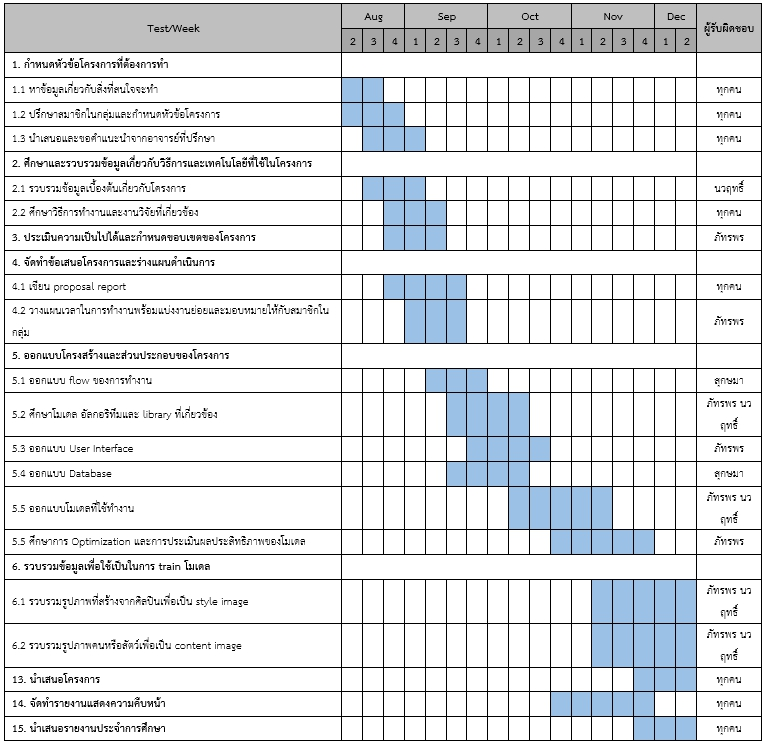
\includegraphics[width=15cm]{./image/plan_table1.jpg}
  \hfill
  \end{tabular}
\caption{ตารางแผนการทำงานภาคการศึกษาที่ 1\centering}
\label{tbl:symbols1}
\end{table}

\newpage

\begin{table}[!h]
  \centering
  \begin{tabular}{c}
  \hfill
  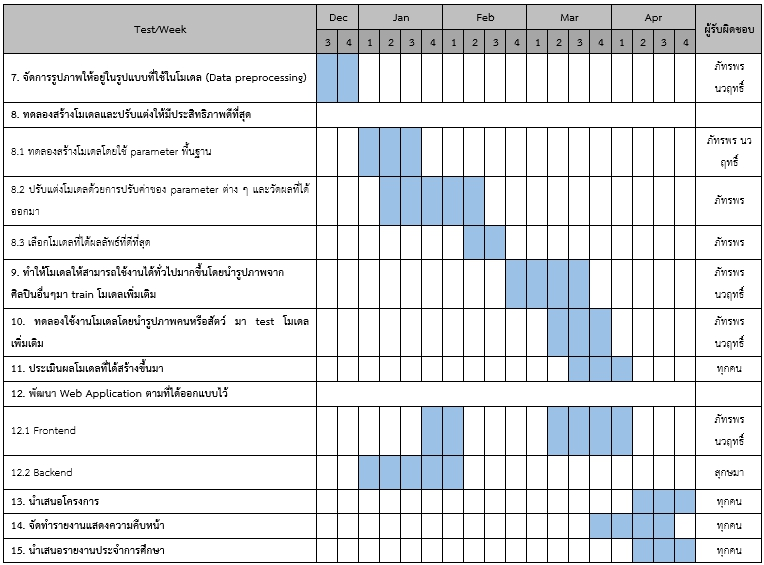
\includegraphics[width=15cm]{./image/plan_table2.jpg}
  \hfill
  \end{tabular}
\caption{ตารางแผนการทำงานภาคการศึกษาที่ 2\centering}
\label{tbl:symbols2}
\end{table}


\section{ผลการดำเนินการ}
\subsection{ผลการดำเนินการในภาคการศึกษาที่1}
\begin{enumerate}
  \item ศึกษาและรวบรวมข้อมูลเกี่ยวกับวิธีการและเทคโนโลยีที่ใช้ในโครงการ
  \item ประเมินความเป็นไปได้และกำหนดขอบเขตของโครงการ
  \item จัดทำข้อเสนอโครงการและร่างแผนดำเนินการ
  \item ออกแบบโครงสร้างและส่วนประกอบของโครงการ
  \item รวบรวมข้อมูลเพื่อใช้เป็นในการ train โมเดล (style image และ content image)
  \item จัดการรูปภาพให้อยู่ในรูปแบบที่ใช้ในโมเดล (Data preprocessing)
  \item สร้างโมเดลโดยใช้ parameter พื้นฐาน
  \item จัดทำรายงานแสดงความคืบหน้า
\end{enumerate}

\newpage
\subsection{ผลการดำเนินการในภาคการศึกษาที่2}
\begin{enumerate}
  \item ทดลองสร้างโมเดลและปรับแต่งให้มีประสิทธิภาพดีที่สุด
  \item ทำโมเดลให้สามารถใช้งานได้ทั่วไปมากขึ้น
  \item ทดลองใช้งานโมเดล
  \item จัดทำ Web application ตามที่ออกแบบไว้
  \item นำเสนอโครงการ
  \item จัดทำรายงานแสดงความคืบหน้า
  \item นำเสนอรายงานประจำการศึกษา
\end{enumerate}


%%%%%%%%%%%%%%%%%%%%%%%%%%%%%%%%%%%%%%%%%%%%%%%%%%%%%%%%%%%%
%%%%%%%%%%%%%%  Literature Review %%%%%%%%%%%%%%%%%%%%%%%%%%
%%%%%%%%%%%%%%%%%%%%%%%%%%%%%%%%%%%%%%%%%%%%%%%%%%%%%%%%%%%%
\chapter{ทฤษฎีความรู้และงานที่เกี่ยวข้อง}
\section{บทนำ}
\par\setlength{\parindent}{5ex}ในบทนี้ อธิบายเกี่ยวกับแนวคิดที่นำมาประยุกต์ใช้ในโครงงาน อัลกอริทึมที่ใช้ในการทำโครงงานคือ VGGNet และมีการพัฒนาโดยใช้ภาษา python นอกจากนี้มีการทบทวนวรรณกรรม ที่จะกล่าวถึงโครงงานที่มีลักษณะเนื้อหาที่เกี่ยวข้องกับการทำโครงการนี้

\section{แนวความคิดทางทฤษฎี}
\subsection{Neural style transfer}
\par\setlength{\parindent}{5ex}Neural Style Transfer \cite{saha2018comprehensive} เป็นกระบวนการที่ใช้ CNNs ในการประมวลผลรูปภาพให้ได้รูปภาพที่เหมือนกับรูปภาพที่ใช้เป็น content image แต่มีรูปแบบหรือลักษณะที่ต่างกันไปตามรูปภาพที่ใช้เป็น style image ดังรูปที่ 2.1


\begin{figure}[!h]
  \centering
  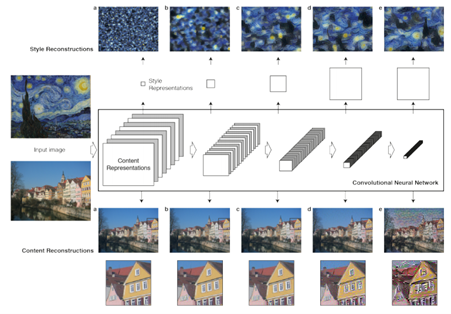
\includegraphics[width=10cm]{./image/unit1.png}
  \caption{แสดงหลักการทำงานของ Neural Style Transfer ที่ใช้ Convolutional Neural Network (CNN) \cite{gatys2015neural} }
  \label{fig:modelcnn}
\end{figure}

\par\setlength{\parindent}{5ex}
ดังรูปที่~\ref{fig:modelcnn} จะเห็นได้ว่า มีการป้อนข้อมูลเป็น content image และ style image 
จากนั้นจะการประมวลผลรูปที่ป้อนเข้ามา โดยจะมี filters ที่ reconstruct 
รูปภาพทั้ง content และ style โดยแสดงให้เห็นกระบวนการต่าง ๆ ใน CNN layer ต่าง ๆ 
ได้แก่ conv1-1(a), conv2-1(b), conv3-1(c), conv4-1(d) และ conv5-1(e) 
ซึ่งจะเห็นว่า ใน layer หลัง ๆ รูปภาพที่ได้รูปภาพที่ได้มีการลดทอนของรูปภาพที่เป็น content 
และมีการเพิ่มส่วนของรูปภาพที่เป็น style เข้าด้วยกัน จนได้ได้รูปภาพที่เหมือนกับรูปภาพที่ใช้เป็น content image 
แต่มีรูปแบบหรือลักษณะที่ต่างกันไปตามรูปภาพที่ใช้เป็น style image

\subsection{Overview of machine learning}
\par\setlength{\parindent}{5ex}Machine learning (ML) เป็นการทำให้คอมพิวเตอร์สามารถเรียนรู้ได้ด้วยตนเอง โดยเริ่มต้นจะต้องสอนให้คอมพิวเตอร์เข้าใจก่อน โดยมีรูปแบบการเรียนรู้ 3 แบบ คือ  Supervised Learning เป็นการเรียนรู้ที่สอนให้คอมพิวเตอร์รู้จักทั้งข้อมูลที่เป็น input และ output ตัวอย่างเช่น การทำนายรูปภาพว่าเป็นหมาหรือแมว ซึ่งต้องสอนให้คอมพิวเตอร์รู้ว่ารูปภาพนี้เป็นหมาหรือแมวก่อนถึงจะเอาไปใช้ได้ เป็นต้น, Unsupervised Learning เป็นการเรียนรู้ที่สอนคอมพิวเตอร์เฉพาะข้อมูลที่เป็น input ไม่มี output ให้โดยจะให้คอมพิวเตอร์เรียนรู้ input ไปเรื่อย ๆ ตัวอย่างเช่น การจัดกลุ่มข้อมูล โดยจะป้อนเฉพาะข้อมูลเข้าไปแล้วคอมพิวเตอร์จะเรียนรู้เองว่า ข้อมูลแบบนี้ควรอยู่กับข้อมูลแบบไหน เป็นต้นและ Reinforcement learning ที่เป็นการเรียนรู้โดยการปฏิสัมพันธ์กับสิ่งแวดล้อมรอบ ๆ โดยถ้าทำถูกต้องจะได้คะแนนเพิ่ม ถ้าทำผิดคะแนนจะลดลง ตัวอย่างเช่น การเดินไปข้างหน้าของหุ่นยนต์ที่จะต้องรู้ก่อนว่า อยู่ตำแหน่งไหน แล้วในตำแหน่งควรเดินไปตำแหน่งไหนต่อไปถึงจะดี เป็นต้น
\par\setlength{\parindent}{5ex}ในขั้นตอนการสร้างโมเดล machine learning จะมีข้อมูล input ที่เกี่ยวข้อง 2 ส่วนคือ training set เป็นชุดข้อมูลที่ใช้สำหรับการสอนโมเดลโดยจะฝึกฝนโมเดลให้ได้ผลลัพธ์ตามชุดข้อมูลที่ป้อนเข้ามา อีกส่วนคือ testing set เป็นชุดข้อมูลที่ใช้ทดสอบการทำงานของโมเดล โดยโมเดลที่ดีจะต้องไม่ทำให้เกิดการ overfitting หรือสามารถทำนายผลลัพธ์ใน training set ได้แม่นยำ แต่ทำนายผลลัพธ์ใน testing set ได้แย่ 
\par\setlength{\parindent}{5ex}เมื่อสอนคอมพิวเตอร์เรียบร้อยแล้ว เมื่อมีข้อมูลใหม่ ๆ เข้า คอมพิวเตอร์ก็สามารถจัดการหรือทำนายข้อมูลนั้นได้เลย ไม่จำเป็นต้องเขียนโปรแกรมใหม่ทุกครั้งที่มีข้อมูลเข้ามา

\subsection{Classical artificial neural networks}
\par\setlength{\parindent}{5ex}
Artificial neural networks(ANN) คือโมเดลทางคณิตศาสตร์หรือโมเดลทางคอมพิวเตอร์ที่จำลองการทำงานของเซลล์ประสาทในสมองมนุษย์ที่มีเซลล์ประสาท(neurons) และจุดประสาทประสาท  ดึงเกิดเป็น ANN ซึ่งมีส่นประกอบในการทำงาน 3 ส่วนหลัก ๆ ดังรูปที่ 2.1 คือ input layer, hidden layer และ output layer ซึ่งการทำงานของ artificial neural networks จะมี 2 ส่วนคือ กระบวนการทำงานไปข้างหน้าหรือ feed forward คือป้อน input เข้าไป แล้วเข้า hidden layer ทำการประมวลผลแล้วได้ค่าออกมาส่งไปที่ output layer และ back propagation หรือกระบวนการทำย้อนกลับโดยจะเป็นการทำย้อนกลับจาก output layer ไป input layer

%%%%%%%no ref
\begin{figure}[!h]
  \centering
  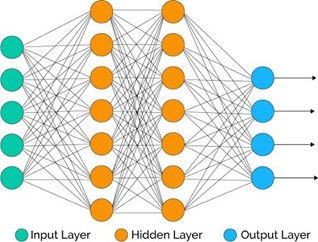
\includegraphics[width=8cm]{./image/unit2.jpg}
  \caption{แสดงส่วนประกอบหลักของ Artificial neural networks}
  \label{fig:modelann}
\end{figure}

\par\setlength{\parindent}{5ex}
ในแต่ละ layer จะมีก้อนกลม ๆ อยู่หรือก็คือ neuron unit อยู่ดังรูปที่ 2.2 ถ้าใน input layer ภายในจะเก็บข้อมูลที่รับเข้ามา แต่ถ้าเป็น hidden layer ภายในจะมีการคำนวณเกิดขึ้นโดยสามารถเพิ่ม hidden layer ได้หลาย layer ตามที่ผู้พัฒนาต้องการได้ ส่วนใน output layer จะมีการทำนายผลออกมาว่า ผลที่ได้เป็นคลาสอะไร


\subsubsection{Neuron unit ใน hidden layer}
\par\setlength{\parindent}{5ex}
ภายใน neuron unit แต่ละตัวใน hidden layer จะมีการคำนวณโดยหลังจากผ่าน input layer เข้ามาจะมีการเพิ่ม weight ให้กับ input neuron unit แต่ละตัว จากนั้นเมื่อเข้า hidden layer ภายในจะรวมผลคูณระหว่าง weight กับ input neuron unit แต่ละตัวเข้าด้วยกันแล้วเข้า step function หรือส่วนใหญ่เรียกว่า activation function จากนั้นจะได้ output ออกมา ดังรูปที่ 2.3

%%%%%%%no ref
\begin{figure}[!h]
  \centering
  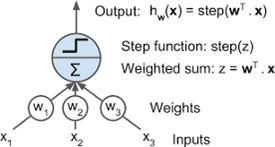
\includegraphics[width=8cm]{./image/neuron_unit.png}
  \caption{แสดงการทำงานภายใน neuron unit \cite{geron2018neura}}
  \label{fig:modelann}
\end{figure}

\subsubsection{Backward propagation}
\par\setlength{\parindent}{5ex}
Backward propagation เป็นกระบวนการทำงานย้อนกลับจาก output layer มา input layer เพื่อปรับค่า weight แต่ละตัวให้ดีขึ้น โดยจะทำไปเรื่อง ๆ จนกว่าจะได้ cost function หรือ error ที่น้อยตามที่ต้องการ 
โดยลักษณะการทำงานของ feed forward กับ back propagation มีลักษณะต่างกันดังรูปที่~\ref{fig:feed-back}

\begin{figure}[!h]
  \centering
  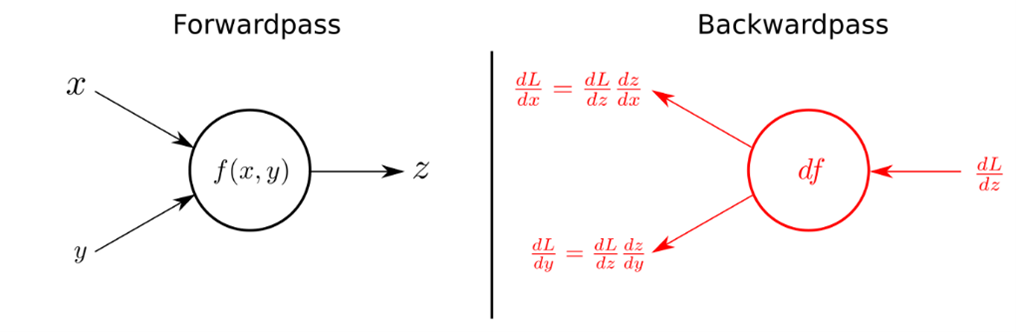
\includegraphics[width=8cm]{./image/feed_back.png}
  \caption{แสดงการทำงานของ feed forward (forwardpass) กับ back propagation (backwardpass)}
  \label{fig:feed-back}
\end{figure}

\par\setlength{\parindent}{5ex}
ในการทำ back propagation จะใช้อัลกอริทึม optimization เพื่อเพิ่มประสิทธิภาพตัวนึงที่ชื่อว่า Gradient descent algorithm [13] ที่จะทำการหา weight ที่ต่ำที่สุดที่จะทำให้โมเดลสามารถทำนายผลได้ดีที่สุด เกิด error น้อย

\subsubsection{Cost function}
\par\setlength{\parindent}{5ex}
Cost function หรือ loss function หรือค่า error ที่เกิดขึ้น ซึ่งจุดมุ่งหมายของโมเดลต่าง ๆ จะเหมือนกันคือ ต้องการให้เกิดค่า error ที่น้อยที่สุดที่เป็นไปได้ ซึ่งการคำนวณค่า error ที่เกิดขึ้นจะใช้การเปรียบเทียบระหว่างผลลัพธ์จริง ๆ ที่ได้มาจากข้อมูลจริงกับผลลัพธ์ที่เกิดจากการทำนายโดยโมเดลมาเทียบกันโดยใช้วิธีต่าง ๆ ตัวอย่างเช่น การคำนวณค่า Mean Squared Error Loss, Mean Absolute Error Loss, Binary Crossentropy Loss, Categorical Crossentropy Loss, Sparse Categorical Crossentropy Loss เป็นต้น ซึ่งการคำนวณแบบต่าง ๆ ก็เหมาะกับปัญหาคนละแบบ ตัวอย่างเช่น Binary Crossentropy Loss ที่เหมาะกับข้อมูลที่มีเพียง 2 คลาส เป็นต้น

\subsection{Convolutional Neural Network (CNN)}
\par\setlength{\parindent}{5ex}
Convolutional Neural Network (CNN) หรือ ConvNet [2,11] เป็นอัลกอริทึม Deep Learning 
ชนิดหนึ่งที่ใช้ประมวลผลรูปภาพ โดยเรียนรู้คุณลักษณะต่าง ๆ ของรูปภาพที่ป้อนเข้าผ่านการใช้ filters 
ซึ่งเป็นการเรียนรู้ลักษณะของรูปภาพ เพื่อแยกแยะว่า รูปภาพที่ป้อนเข้ามาเป็นรูปอะไรดังรูปที่~\ref{fig:pic-cnn}

\begin{figure}[!h]
  \centering
  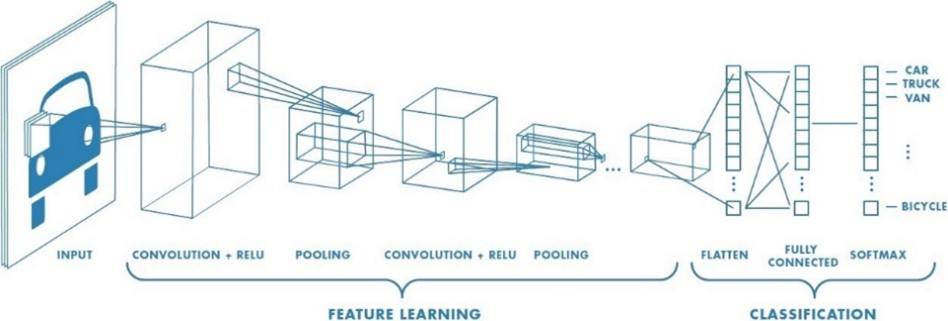
\includegraphics[width=12cm]{./image/cnn.jpg}
  \caption{แสดงให้เห็นถึงกระบวนการทำงานของ CNN ที่มีการเรียนรู้ 2 ส่วนคือ feature learning ซึ่งมี convolution layer และ pooling layer ประกอบกัน และ classification ซึ่งมี fully connected layer มาเกี่ยวข้อง}
  \label{fig:pic-cnn}
\end{figure}


\subsubsection{Input data}
\par\setlength{\parindent}{5ex}
ข้อมูลที่เข้ามาประมวลใน CNN เป็นรูปภาพซึ่งมีหลากหลายรูปแบบที่เป็นขาวดำหรือ Grayscale, รูปภาพสีแบบ RGB, HSV หรือ CMYK เป็นต้น ซึ่งโดยส่วนใหญ่เป็นรูปภาพสีแบบ RGB ซึ่งเมื่อรับ input เข้ามาจะถูกแบ่งสีออกเป็น channels คือ Red(R) , Green(G) และ Blue(B) และแปลงขนาดความกว้างและความยาวของรูปภาพให้เป็น pixels 
ทำให้อยู่ในรูป heights*weights*จำนวนของ channels ดังรูปที่~\ref{fig:rgb-layer}

\begin{figure}[!h]
  \centering
  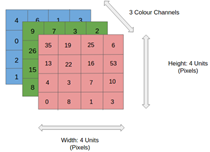
\includegraphics[width=8cm]{./image/unit3.png}
  \caption{แสดงให้เห็นถึงลักษณะของ input data ที่มีการแบ่งชั้นสีเป็น 3 channels ซึ่งจากรูปนี้จะมีขนาดของรูปเป็น 4*4*3 RGB Image}
  \label{fig:rgb-layer}
\end{figure}

\subsubsection{Convolution layer}
\par\setlength{\parindent}{5ex}
ในส่วนของ convolutional layer จะมี filter หรือ Kernel (K) ซึ่งเป็น matrix ขนาดต่าง ๆ ใช้สำหรับ map กับข้อมูลที่เข้ามา และมี stride ที่ใช้สำหรับบอกว่าต้องขยับ filter ไปกี่ pixels โดย filters จะเคลื่อนที่ไปเรื่อย ๆ จนผ่านครบทุก pixels ในข้อมูลที่เข้ามา และนอกจากนี้จะมีการใช้ non-linear functions เพื่อ scale ข้อมูลที่เข้ามาไม่ให้ติดลบซึ่งเหมาะกับการเรียนรู้ใน CNNs โดยตัวที่นิยมใช้คือ Rectified Linear Unit (ReLU) ที่มีฟังก์ชันคือ ƒ(x) = max(0,x) 

\subsubsection{Pooling layer}
\par\setlength{\parindent}{5ex}
ในส่วนของ pooling layer จะทำงานต่อจาก convolution layer โดยจะทำการดึงข้อมูลออกมาหลังจากที่มีการทำ filter แต่ละครั้ง ออกมาเป็นข้อมูลที่ออกมา ณ ตำแหน่งนั้น ๆ ที่มีการทำ filter ทำให้สามารถดึงลักษณะสำคัญของข้อมูลที่เข้ามาได้ ตัวอย่างเช่น ขอบ สี รูปทรง เป็นต้น และยังทำให้ขนาดข้อมูลที่ได้ออกมามีขนาดเล็กลงเมื่อเทียบกับข้อมูลที่เข้ามา โดย pooling มี 3 แบบ คือ min pooling, max pooling และ average pooling ซึ่ง convolution layer กับ pooling layer จะทำงานคู่กัน ซึ่งใน CNN จะมีกี่ layer นั้นขึ้นอยู่กับความซับซ้อนของรูปภาพ

\subsubsection{Fully connected layer}
\par\setlength{\parindent}{5ex}
เมื่อทำ feature learning โดยใช้ convolution layer กับ pooling layer แล้ว output ที่ได้จะอยู่ในรูปแบบที่เป็น 3 ชั้นหรือมี 3 มิติอยู่ จะมีการทำ flatten ก่อนเพื่อให้อยู่ในรูปแบบที่เป็น 1 มิติ เพื่อที่จะได้สามารถเข้าไปใน fully connected layer ได้ โดยใน fully connected layer มีการใช้ softmax classification ที่ใช้แยกว่าข้อมูล input ที่เข้ามาเป็นรูปอะไรโดยแสดงผลเป็นความเป็นไปได้ที่เป็นรูปต่าง ๆ 

\subsection{Transfer Learning}
\par\setlength{\parindent}{5ex}
Transfer Learning เป็นการเรียนรู้ที่เป็นที่นิยมในการทำ machine learning(ML) โดยเป็นการนำโมเดลที่มีคนสร้างมาก่อนที่เหมาะกับงานหนึ่ง ๆ มาประยุกต์ใช้กับงานอื่นโดยไม่จำเป็นต้องสอนโมเดลใหม่ทั้งหมด 
ทำให้สามารถลดเวลาประมวลผลและเวลาในการสอนโมเดลได้ ดังรูปที่~\ref{fig:ml-tl}

\newpage

\begin{figure}[!h]
  \centering
  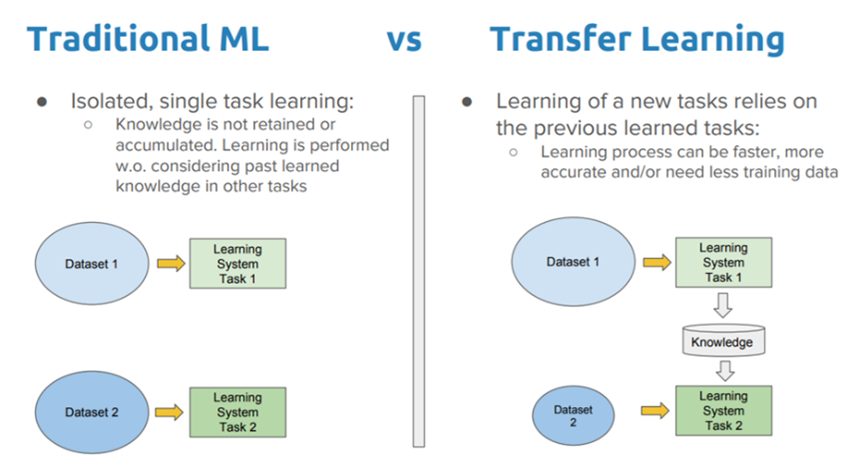
\includegraphics[width=12cm]{./image/unit4.png}
  \caption{แสดงให้เห็นถึงการเปรียบเทียบการทำงานระหว่าง traditional ML กับ transfer learning ที่มีรูปแบบการทำงานที่ต่างกัน \cite{brownlee2017gentle}}
  \label{fig:ml-tl}
\end{figure}

\par\setlength{\parindent}{5ex}
โดยในการทำ transfer learning มีอยู่ 2 รูปแบบ คือ develop model ซึ่งเป็นการนำโมเดลนั้นมาแก้ไขและพัฒนาให้ดีกว่าเดิมให้เหมาะกับงานที่โมเดลนั้นสร้างมาใช้และจึงนำไปใช้กับงานอื่น ๆ ส่วนอีกรูปแบบคือ pre-trained model ซึ่งเป็นการนำโมเดลไปใช้กับงานอื่นเลย โดยส่นใหญ่จะใช้ pre-trained model เป็นหลัก 
\par\setlength{\parindent}{5ex}
สำหรับการทำ transfer learning ที่เกี่ยวกับรูปภาพ\cite{8636278}\cite{sarkar2018comprehensive}มีการสร้างโมเดลสำหรับ ImageNet ที่มีรูปภาพกว่า 1.4 ล้านรูปและมากกว่า 1,000 คลาสที่เป็นความท้าทายสำหรับการทำ image classification ทำให้มีองค์การวิจัยต่าง ๆ มีการพัฒนาโมเดลขึ้นมาสำหรับแก้ปัญหานี้ และได้เปิดให้คนทั่วไปสามารถเอาไปใช้ได้ ตัวอย่างเช่น โมเดล VGG ของ Oxford, โมเดล Inception ของ Google และโมเดล ResNet ของ Microsoft เป็นต้น

\subsubsection{VGGNet}
\par\setlength{\parindent}{5ex}
Visual Geometry Group (VGG) เป็น CNN สำหรับจดจำรูปภาพ ซึ่งสถาปัตยกรรมของ VGG จะประกอบไปด้วยบล็อค 
แต่ละบล็อกจะเป็น 2 มิติ คือ Convolution layer และ Pooling layer แนวความคิดนี้ถูกพัฒนาโดย 
Simonyan \& Zisserman จาก Oxford Robotics Institute ซึ่ง VGG นั้นมีโมเดล 2 ตัวคือ VGG16 และ VGG19 
ซึ่งเลข 16 และ เลข 19 นั้นมาจากคือจำนวนของ hidden layer สำหรับ VGG16 จะประกอบไปด้วยบล็อคของ 
convolutional layer และ Pooling ทั้งหมด 13 layers และ Fully connected layer 3 layers ส่วน VGG 19 
นั้นคือ VGG16 ที่มีบล็อคของ convolutional layer เพิ่มมาอีก 3 layers  ดังรูปที่ ~\ref{fig:vgg16-19} 

\begin{figure}[!h]
  \centering
  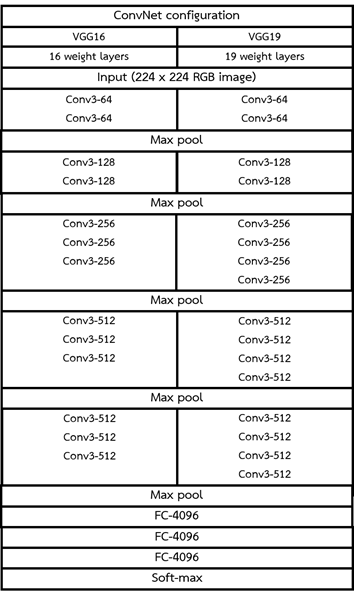
\includegraphics[width=8cm]{./image/vgg16-19.png}
  \caption{แสดงสถาปัตยกรรมของ VGG16 และ VGG19}
  \label{fig:vgg16-19}
\end{figure}

\newpage

\subsection{Web Application}
\par\setlength{\parindent}{5ex}
Web Application เป็นซอฟต์แวร์นึงที่สามารถเข้าถึงผ่าน browser ใดก็ได้ โดยที่ผู้ใช้ไม่ต้องดาวน์โหลดก่อนใช้งานเพราะสามารถเข้าถึงได้ผ่าน network ซึ่ง Web Application นั้นออกแบบมาให้สามารถมีปฏิสัมพันธ์กับผู้ใช้ได้ ไม่ใช่แค่การดูข้อมูลต่าง ๆ แต่สามารถจัดการหรือใช้งานได้ ซึ่งผู้ใช้หลายคนสามารถเข้าถึงพร้อมกัน
\par\setlength{\parindent}{5ex}
หลักการทำงานของ web Application คือ ผู้ใช้งานติดต่อสื่อสารกับ web application ผ่าน frontend หรือ client-side ซึ่ง frontend จะมีการเรียกใช้หรือดึงข้อมูลออกมาจาก backend หรือ server-side ผ่าน http request ที่ถูกเรียกใช้โดยผู้ใช้งาน ภายใน backend จะมี web server, database 
และไฟล์อื่น ๆ เก็บไว้ ดังรูปที่~\ref{fig:webapp} 

%%%%no ref
\newpage
\begin{figure}[!h]
  \centering
  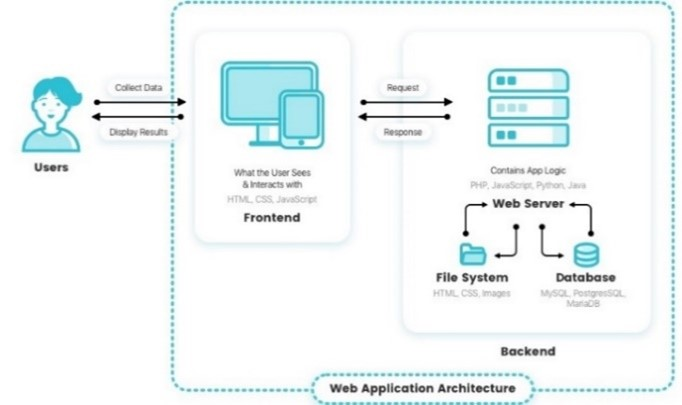
\includegraphics[width=8cm]{./image/webapp.jpg}
  \caption{แสดงหลักการทำงานของ web application}
  \label{fig:webapp}
\end{figure}

\subsection{Development Tools}
\subsubsection{Python}
\par\setlength{\parindent}{5ex}
Python เป็นภาษาที่ใช้ในการเขียนโปรแกรม ซึ่งได้รับความนิยมเป็นอย่างมาก เนื่องจากเป็นภาษาที่เรียนรู้ง่าย ใช้งานง่ายและมีประสิทธิภาพสูง ถูกพัฒนาขึ้นโดย Guido van Rossum ในปี ค.ศ. 1991 ซึ่งสามารถทำงานบนแพลตฟอร์ต่าง ๆ ได้หลากหลาย มีไวยากรณ์ที่เข้าใจง่ายสามารถเขียนได้ทั้งแบบเชิงวัตถุ object-oriented หรือแบบฟังก์ชัน functional และรันบน interpreter system ซึ่งประมวลผลได้อย่างรวดเร็วและมี library หลากหลายให้ใช้งาน

\subsubsection{Hypertext Markup Language (HTML)}
\par\setlength{\parindent}{5ex}
Hypertext Markup Language (HTML) เป็นภาษาคอมพิวเตอร์ที่ใช้ในการแสดงผลของข้อความ รูปภาพหรือวัตถุอื่น ๆ บนหน้าเว็บไซต์ โดยมีโครงสร้างการเขียนที่อาศัย tag ควบคุมซึ่งถูกพัฒนาโดย World Wide Web Consortium (W3C) โดยออกแบบมาให้สามารถทำความเข้าใจและเรียนรู้ง่าย โดยใน tag ต่าง ๆ จะแตกต่างกันไปแต่มีส่วนประกอบหลักที่เหมือนกันคือ เครื่องหมาย “<>” และมีชื่ออยู่ตรงกลางเครื่องหมายนั้น ตัวอย่างเช่น <head> </head> เป็นต้น

\subsubsection{Cascading Style Sheets (CSS)}
\par\setlength{\parindent}{5ex}
Cascading Style Sheets (CSS) หรือ Style Sheets เป็นภาษาคอมพิวเตอร์ตัวนึง ที่ใช้สำหรับกำหนดรูปแบบการแสดงผลของเอกสาร html อันได้แก่ สีข้อความ ขนาดข้อความ ประเภทตัวอักษร ขนาดรูปภาพ การจัดวางข้อความ สีพื้นหลัง เป็นต้น

\subsubsection{JavaScript}
\par\setlength{\parindent}{5ex}
JavaScript เป็นภาษาคอมพิวเตอร์ชนิดหนึ่งที่ใช้ร่วมกับเอกสาร html เพื่อให้เว็บไซต์มีการเคลื่อนไหวเพื่อตอบสนองต่อการใช้งานของผู้ใช้มากขึ้น โดยมีลักษณะการทำงานคือ แปลความและดำเนินงานไปทีละคำสั่ง หรือ object-oriented programming ซึ่งดำเนินการโดย browser เป็น client-side script ทำให้สามารถใช้งานกับ server ใดก็ได้ โดย javaScript นี้สามารถเขียนเพื่อเปลี่ยนแปลง html element ได้ สามารถตอบสนองกับผู้ใช้และตรวจสอบข้อมูล รวมไปถึงสร้าง cookies ที่ใช้เก็บข้อมูลในคอมพิวเตอร์ของผู้ใช้ได้

\subsubsection{Pytorch}
\par\setlength{\parindent}{5ex}
Pytorch เป็น Deep learning library ที่ Facebook เป็นคนพัฒนาขึ้นด้วยภาษา python โดยดัดแปลงมาจาก library torch ที่ถูกใช้ในภาษา Lua มาก่อน โดยจะมองข้อมูลให้อยู่ในรูปของ tensor ซึ่งเป็นการเก็บข้อมูลหลายมิติแบบ arrays ทำให้สามารถใช้ numpy ในการคำนวณได้เลย และมีการเตรียม neural network แบบต่าง ๆ ไว้ให้ผู้พัฒนาสามารถนำไปพัฒนาต่อได้อย่างรวดเร็ว และยังสามารถใช้ GPU เข้ามาช่วยในการคำนวณได้ ทำให้สามารถประมวลผลได้เร็วขึ้น

\subsubsection{Django}
\par\setlength{\parindent}{5ex}
Django เป็น high-level python web framework ที่ช่วยให้ผู้พัฒนาสามารถสร้าง web application ได้อย่างรวดเร็ว ซึ่งจุดเด่นของ Django คือ มีระบบ admin มาให้ทำให้ผู้พัฒนาไม่จำเป็นสร้างใหม่เอง สามารถใช้งานกับโปรแกรม editor ได้หลากหลายตามที่ผู้พัฒนาถนัด มีเครื่องมือที่ช่วยให้ผู้พัฒนาสามารถขึ้นโครงโปรแกรมได้อย่างรวดเร็ว ตัวอย่างเช่น ระบบการจัดการข้อมูล(models), ระบบแสดงผล(views), ระบบการเข้าใช้งานของผู้ใช้, ระบบการจัดการผู้ใช้งาน เป็นต้น รวมทั้งมี Django REST Framework ที่ช่วยให้ผู้พัฒนาสามารถสร้าง API เพื่อให้ในส่วน frontend สามารถติดต่อกับส่วน backend ได้อย่างสะดวก รวดเร็ว

\par\setlength{\parindent}{5ex}
หลักการของ Django คือ 1 Project มี 1 app โดย 1 app คือ 1 module ในเว็บไซต์ ในการสร้าง Django Project [9] ผู้ใช้จะได้ไฟล์หลายไฟล์ดังรูปที่ 2.10 ซึ่งไฟล์หลัก ๆ ประกอบไปด้วย
\begin{enumerate}
  \item manage.py ที่เป็นไฟล์ script สำหรับรันคำสั่งต่าง ๆ ที่เกี่ยวข้องกับ Django
  \item _init_.py เป็นไฟล์ initial หรือไฟล์เปล่าที่มีไว้สำหรับเก็บ package ของ python
  \item setting.py เป็นไฟล์ที่ใช้ตั้งค่า project ตัวอย่างเช่น การตั้งค่า app, การตั้งเวลา, การตั้งค่า path เป็นต้น
  \item urls.py เป็นไฟล์ที่มีไว้สำหรับเก็บ HTTP Request หรือ url pattern ที่เป็นการ routing ภายใน Django project
  \item wsgi.py เป็นไฟล์ที่เก็บข้อมูลสำหรับการ deployment หรือการ production ให้ผู้ใช้ใช้งาน
\end{enumerate}


\newpage
\begin{figure}[!h]
  \centering
  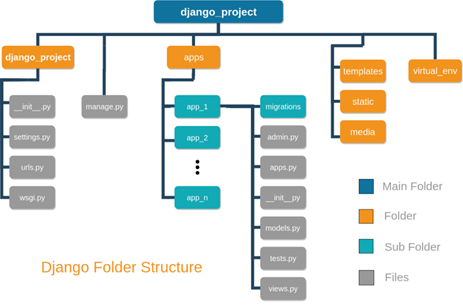
\includegraphics[width=8cm]{./image/django.png}
  \caption{แสดงโครงสร้างโฟลเดอร์ของ Django project}
  \label{fig:django}
\end{figure}

\par\setlength{\parindent}{5ex}
และ Django เป็น model-view-template (MVT) ซึ่งมีกระบวนการทำงานหลัก ๆ 3 ส่วน ดังรูปที่ 2.11 คือ Model ที่เก็บข้อมูลของ application, View สำหรับประมวลผลคำสั่งหรือข้อมูลต่าง ๆ แล้วส่งไปที่ Template, Template คือหน้า application ที่ใช้แสดงผลข้อมูลที่ผ่านการประมวลผลจาก view ร่วกับ html โดยมีการใช้ http request และ http response ในการติดต่อกับส่วนต่าง ๆ 










%%%%%%%%%%%%%%%%%%%%%%%%%%%%%%%%%%%%%%%%%%%%%%%%%%%%%55
%%%%%%%%%%%%%%%%%%%%%%%%%%%%%%%%%%%%%%%%%%%%%%%%%%%%%
%%%%%%%%%%%%%%%%%%%%%%%%%%%%%%%%%%%%%%%%%%%%%%%%%%%%%
\chapter{วิธีการดำเนินงาน}

Explain the design (how you plan to implement your work) of your project. Adjust the section titles below to suit the types of your work. Detailed physical design like circuits and source codes should be placed in the appendix.

\section{ข้อกำหนดและความต้องการของระบบ}

\section{สถาปัตยกรรมระบบ}

\begin{table}[!h]
\centering
\caption{test table x1}\label{tbl:symbols}
\begin{tabular}{@{}p{0.07\textwidth}|p{0.7\textwidth}p{0.1\textwidth}}\hline
\multicolumn{2}{l}{\textbf{SYMBOL}}  & \textbf{UNIT} \\ \hline 
$\alpha$ & Test variable\hfill & m$^2$ \\
$\lambda$ & Interarrival rate\hfill &  jobs/second\\
$\mu$ & Service rate\hfill & jobs/second \\ \hline
\end{tabular}
%\begin{tabular}{c|c} \hline
% $\alpha$ & $\beta$ \\ \hline
% $\delta$ & $\mu$ \\ \hline
%\end{tabular}
\end{table}



\section{Hardware Module 1}
\subsection{Component 1}
\subsection{Logical Circuit Diagram}

\section{Hardware Module 2}
\subsection{Component 1}
\subsection{Component 2}

\section{Path Finding Algorithm}

\section{Database Design}

\section{UML Design}

\section{GUI Design}

\section{การออกแบบการทดลอง}
\subsection{ตัวชี้วัดและปัจจัยที่ศึกษา}
\subsection{รูปแบบการเก็บข้อมูล}




%%%%%%%%%%%%%%%%%%%%%%%%%%%%%%%%%%%%%%%%%%%%%%%%%%%%%%%%%%%%%%
%%%%%%%%%%%%%%%%%%%% Experiments %%%%%%%%%%%%%%%%%%%%%%%%%%%%%
%%%%%%%%%%%%%%%%%%%%%%%%%%%%%%%%%%%%%%%%%%%%%%%%%%%%%%%%%%%%%%%
\chapter{ผลการดำเนินงาน}

You can title this chapter as \textbf{Preliminary Results} ผลการดำเนินงานเบื้องต้น or \textbf{Work Progress} ความก้าวหน้าโครงงาน for the progress reports. Present implementation or experimental results here and discuss them.
ใส่เฉพาะหัวข้อที่เกี่ยวข้องกับงานที่ทำ 

\section{ประสิทฺธิภาพการทำงานของระบบ} 
\section{ความพึงพอใจการใช้งาน}
\section{การวิเคราะห์ข้อมูลและผลการทดลอง}

%%%%%%%%%%%%%%%%%%%%%%%%%%%%%%%%%%%%%%%%%%%%%%%%%%%%%%%%%%%%%%%
%%%%%%%%%%%%%%%%%%%% Conclusions %%%%%%%%%%%%%%%%%%%%%%%%%%%%%
%%%%%%%%%%%%%%%%%%%%%%%%%%%%%%%%%%%%%%%%%%%%%%%%%%%%%%%%%%%%%%%
\chapter{บทสรุป}

This chapter is optional for proposal and progress reports but 
is required for the final report.

\section{สรุปผลโครงงาน}
สรุปว่าโครงงานบรรลุตามวัตถุประสงค์ที่ตั้งไว้หรือไม่ อย่างไร 

\section{ปัญหาที่พบและการแก้ไข}
State your problems and how you fixed them.

\section{ข้อจำกัดและข้อเสนอแนะ}
ข้อจำกัดของโครงงาน What could be done in the future to make your projects better.

%%%%%%%%%%%%%%%%%%%%%%%%%%%%%%%%%%%%%%%%%%%%%%%%%%%%%%%%%%%%%%%
%%%%%%%%%%%%%%%%%%%% Bibliography %%%%%%%%%%%%%%%%%%%%%%%%%%%%%
%%%%%%%%%%%%%%%%%%%%%%%%%%%%%%%%%%%%%%%%%%%%%%%%%%%%%%%%%%%%%%%

%%%% Comment this in your report to show only references you have
%%%% cited. Otherwise, all the references below will be shown.
\nocite{*}
%% Use the kmutt.bst for bibtex bibliography style 
%% You must have cpe.bib and string.bib in your current directory.
%% You may go to file .bbl to manually edit the bib items.
\bibliographystyle{kmutt}
\bibliography{string,cpe}

%%%%%%%%%%%%%%%%%%%%%%%%%%%%%%%%%%%%%%%%%%%%%%%%%%%%%%%%%%%%%%%
%%%%%%%%%%%%%%%%%%%%%%%% Appendix %%%%%%%%%%%%%%%%%%%%%%%%%%%%%
%%%%%%%%%%%%%%%%%%%%%%%%%%%%%%%%%%%%%%%%%%%%%%%%%%%%%%%%%%%%%%%
\appendix{ชื่อภาคผนวกที่ 1}
\noindent{\large\bf ใส่หัวข้อตามความเหมาะสม} \\

This is where you put hardware circuit diagrams, detailed experimental data in tables or source codes, etc.. \\ \bigskip



This appendix describes two static allocation methods for fGn (or fBm)
traffic. Here, $\lambda$ and $C$ are respectively the traffic arrival
rate and the service rate per dimensionless time step. Their unit are
converted to a physical time unit by multiplying the step size
$\Delta$. For a fBm self-similar traffic source,
%Norros~\cite{norros95} provides its EB as
\begin{equation}\label{eq:norros}
  C = \lambda + (\kappa(H)\sqrt{-2\ln\epsilon})^{1/H}a^{1/(2H)}x^{-(1-H)/H}\lambda^{1/(2H)}
\end{equation}
where $\kappa(H) = H^H(1-H)^{(1-H)}$. Simplicity in the calculation is
the attractive feature of (\ref{eq:norros}).

The MVA technique developed in~\cite{kim01} so far provides the most
accurate estimation of the loss probability compared to previous
bandwidth allocation techniques according to simulation results.
Consider a discrete-time queueing system with constant service rate
$C$ and input process $\lambda_n$ with $\mathbb{E}\{\lambda_n\} =
\lambda$ and $\mathrm{Var}\{\lambda_n\} = \sigma^2$.  Define $X_n \equiv
\sum_{k=1}^n \lambda_k - Cn$.  The loss probability due to the MVA
approach is given by
\begin{equation}\label{eq:loss_mva}
  \varepsilon \approx \alpha e^{-m_x/2}
\end{equation}
where
\begin{equation}\label{eq:mx}
m_x = \min_{n \geq 0} \frac{((C-\lambda)n + B)^2}{\mathrm{Var}\{X_n\}} =
\frac{((C-\lambda)n^\ast + B)^2}{\mathrm{Var}\{X_{n^{\ast}}\}}
\end{equation} 
and 
\begin{equation}\label{eq:alpha}
  \alpha =
  \frac{1}{\lambda\sqrt{2\pi\sigma^2}}\exp\left(\frac{(C-\lambda)^2}{2\sigma^2}\right)
  \int_C^\infty (r-C)\exp\left(\frac{(r-\lambda)^2}{2\sigma^2}\right)\, dr
\end{equation}
For a given $\varepsilon$, we numerically solve for $C$ that satisfies
(\ref{eq:loss_mva}). Any search algorithm can be used to do the task.
Here, the bisection method is used.  

Next, we show how $\mathrm{Var}\{X_n\}$ can be determined.  Let
$C_{\lambda}(l)$ be the autocovariance function of $\lambda_n$.  The
MVA technique basically approximates the input process $\lambda_n$
with a Gaussian process, which allows $\mathrm{Var}\{X_n\}$ to be
represented by the autocovariance function.  In particular, the
variance of $X_n$ can be expressed in terms of $C_{\lambda}(l)$ as
\begin{equation}
  \mathrm{Var}\{X_n\} = nC_{\lambda}(0) + 2\sum_{l=1}^{n-1} (n-l)C_{\lambda}(l)
\end{equation} 
Therefore, $C_{\lambda}(l)$ must be known in the MVA technique, either
by assuming specific traffic models or by off-line analysis in case of
traces.  In most practical situations, $C_{\lambda}(l)$ will not be
known in advance, and an on-line measurement algorithm developed
in~\cite{eun01} is required to jointly determine both $n^\ast$ and
$m_x$. For fGn traffic, $\mathrm{Var}\{X_n\}$ is equal to $\sigma^2
n^{2H}$, where $\sigma^2 = \mathrm{Var}\{\lambda_n\}$, and we can find
the $n^\ast$ that minimizes (\ref{eq:mx}) directly. Although $\lambda$
can be easily measured, it is not the case for $\sigma^2$ and $H$.
Consequently, the MVA technique suffers from the need of prior
knowledge traffic parameters.


%%%%%%%%%%%%%%%%%%%%%%%%%%%%%%%%%%%%%%%%%%%%%%%%%%%%%%%%%%
%%%%%%%%%%%%%%% The 2nd appendix %%%%%%%%%%%%%%%%%%%%%%%%%%
%%%%%%%%%%%%%%%%%%%%%%%%%%%%%%%%%%%%%%%%%%%%%%%%%%%%%%%%%%
\appendix{ชื่อภาคผนวกที่ 2}
\noindent{\large\bf ใส่หัวข้อตามความเหมาะสม} \\

Next, we show how $\mathrm{Var}\{X_n\}$ can be determined.  Let
$C_{\lambda}(l)$ be the autocovariance function of $\lambda_n$.  The
MVA technique basically approximates the input process $\lambda_n$
with a Gaussian process, which allows $\mathrm{Var}\{X_n\}$ to be
represented by the autocovariance function.  In particular, the
variance of $X_n$ can be expressed in terms of $C_{\lambda}(l)$ as
\begin{equation}
  \mathrm{Var}\{X_n\} = nC_{\lambda}(0) + 2\sum_{l=1}^{n-1} (n-l)C_{\lambda}(l)
\end{equation} 

\noindent{\large\bf Add more topic as you need} \\

Therefore, $C_{\lambda}(l)$ must be known in the MVA technique, either
by assuming specific traffic models or by off-line analysis in case of
traces.  In most practical situations, $C_{\lambda}(l)$ will not be
known in advance, and an on-line measurement algorithm developed
in~\cite{eun01} is required to jointly determine both $n^\ast$ and
$m_x$. For fGn traffic, $\mathrm{Var}\{X_n\}$ is equal to $\sigma^2
n^{2H}$, where $\sigma^2 = \mathrm{Var}\{\lambda_n\}$, and we can find
the $n^\ast$ that minimizes (\ref{eq:mx}) directly. Although $\lambda$
can be easily measured, it is not the case for $\sigma^2$ and $H$.
Consequently, the MVA technique suffers from the need of prior
knowledge traffic parameters. 





\end{document}
